\chapter{Background}

% Introduce what is planning under uncertainty
Planning and reasoning under uncertainty is central to robotic and artificial intelligence research and has 
been an active area of research for decades. It is an umbrella term which touches a
wide spectrum of fields: \textit{economics}, \textit{psychology}, \textit{cognitive science}, \textit{neuroscience},
\textit{robotics} and \textit{artificial intelligence}. The work in this thesis relies on results  and assumptions 
made in cognitive and neuroscience with respect to our beliefs and how we act given them. We complement 
these results by introducing them in a new light to the field of robotics and demonstrate how the human reasoning and belief system 
can be used in situations where the state space is partially observable. The second main theme our work builds on is 
state space estimation. The third component acting given uncertainty in robotics. We make use of results from all 
three fields. We provide a background overview of acting under uncertainty and situate our work within the state of the 
art.

This chapter unfolds as follows: 



\section{Planning and Uncertainty}
% What is the the reasoning under uncertainty planning problem
% What are all the assumptions which can be made regading the belief

\subsection{The problem}

Planning, control and decision theory are concerned with finding a set of actions which will lead to the 
successful outcome of a problem being considered; this the most generic definition. There are two 
key attributes which can make this problem difficult: stochastic actions and latent states. Stochastic 
actions, when applied in the same state will not always lead to the same outcome. This type of uncertainty 
can arise from many sources; the outcome of chaotic actions are impossible to predict with certainty, 
think of throwing a die or flipping a coin; In outdoor robotics the terrain might lead to slippage, causing 
the robot to skid or underwater currents might drastically offset the position of an UAV; In articulated 
robots the friction between joints can accumulate to a large error in the end-effector position (especially true 
for cable driven robots). 
The second source of uncertainty is when the underlying state is partially known, in the sense that we do not 
have all the necessary information to reliably determine the state beyond reasonable doubt. In robotics this 
uncertainty can arise from inadequate or noisy sensors. If the environmental conditions in which the robot 
is located is humid, misty or dark. It can make it difficult for the robot ascertain its position and 
makes it difficult to plan how to achieve a given objective.

The uncertainty of the state and actions have to be quantified. The predominant approach 
is to  represent them by probabilities. For instance the application of a forward action (for a wheeled robot) 
will result in a new position further ahead and a position to the right (due to slippage) with some probability.
An observation through the robots sensors will result in probability distribution over the robots probable location.
Given this quantification of action and observation uncertainty in terms of a probability distribution over the state, 
the agent must now take actions towards accomplishing its goal. To take a decision the agent must assign a utility 
to the outcome of his actions. The utility is to indicate a preference over the outcomes and when combined with 
probabilities leads to decision theory. 


%How is the uncertainty quantified ? Answer: probability theory
%How does the agent make a decision ? He must assigned a preference to the outcome of various actions
%Utility theory and combined with probability lead to decision theory.

% Speak about the historical context of plannig un
% Uncertainty and rational actions


\begin{figure}[h]
 \centering
 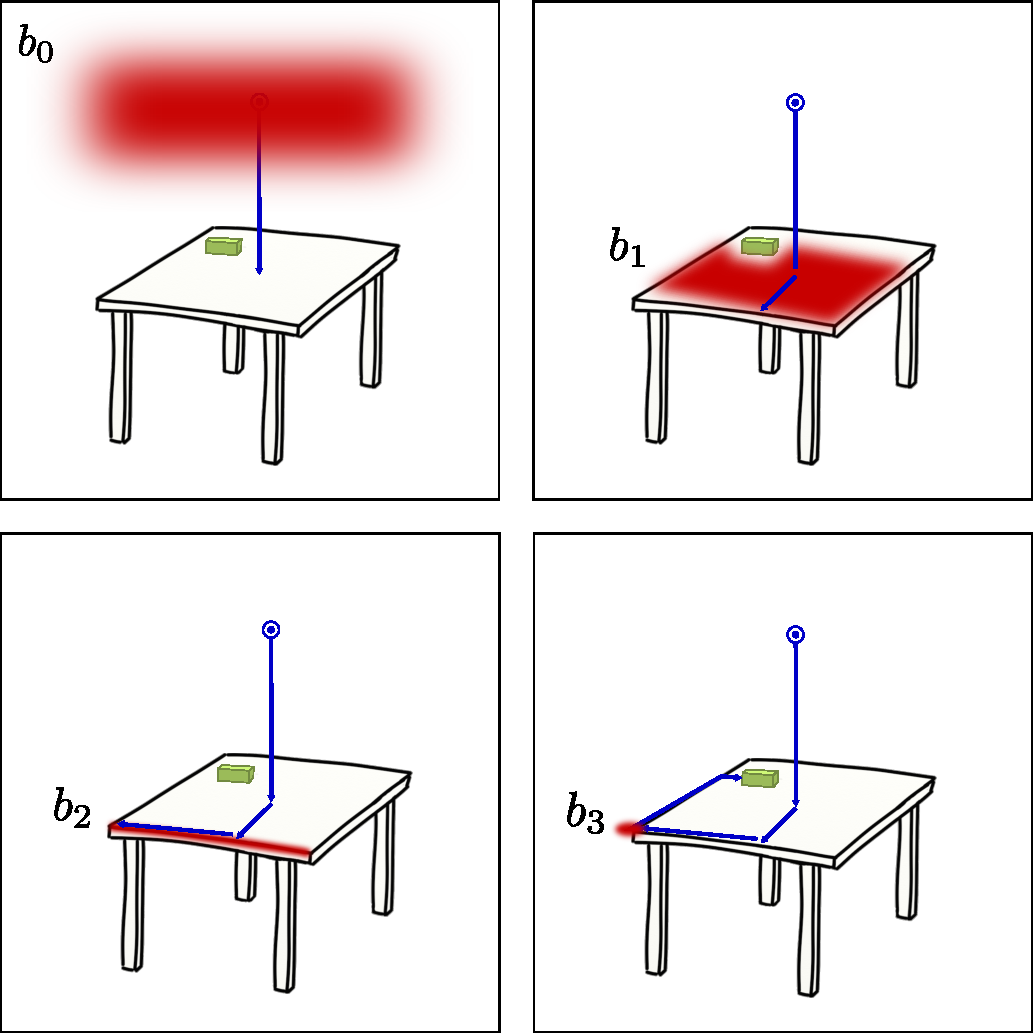
\includegraphics[width=0.8\textwidth]{/home/guillaume/Documents/Thesis/ch2-Background/Figures/reasoning_uncertainty_concept1.pdf}
 \caption{ad}
\end{figure}


% 1) POMDP
%	Based on Markove Decision Process
%	Talk about background in Optimal control and decision theor
%	Assume convex cost function, can be in feature space
%	 1.1) Approximatee POMDP
%	 1.2) MC-POMDP


\subsection{Belief space}

% 2) Belief space (planning)
%	belief roadmap (assumption on the noise)
%
% 3)  Belief space (optimal control)
%
%
\subsection{Summary}
% 4) Assumptions about motion noise and observation 
%
%

% Policy search
\cite{Sol_POMDP_Policy_space_1998}

\subsubsection{Tree search}

\subsubsection{Planning}
$b = (\mu,\Sigma)$
\cite{Quadrator_2008},\cite{BelRoadMap_2009}


\subsubsection{Optimal control}
$b = (\mu,\Sigma)$
 
\cite{Erez10ascalable},
\cite{mc_update_ppomdps}, 
\cite{Platt-RSS-10}

 
% Continous

Optimal control methods represent the belief by a Gaussian function 


\cite{Bayesian_explor_exploit_2009},\cite{Spaan05icra},\cite{Thrun_2005}
 
% Sample based replanning

\cite{Rand_belief_space_replanning}
 
 
 % Online vs Offline methods
 \cite{Ross08onlineplanning}
 
 % Macro-Actions
 \cite{Macro_uncertainty_2011}


\section{Human and uncertainty}

%	Decision Theory & optimal research
%	Theory of Mind




% What did we start off with and where are we now. What are the current achievements or reasonin under uncertainty and 
% what are still the open problem.

% It is a very broad area of research since we borrow elements from the human belief system and theory of mind. 
% 
%	1) Acting under uncertainty is not an easy problem. 
%
%	
%
%
%	--- We are all about how to reason and act given uncertainty. 
%	Decision theory and operational research (historical context)
%	Bayesian Theory of Mind (Cognitive side of things). We are risk averse etc..
%



\begin{figure}[h]
 \centering
 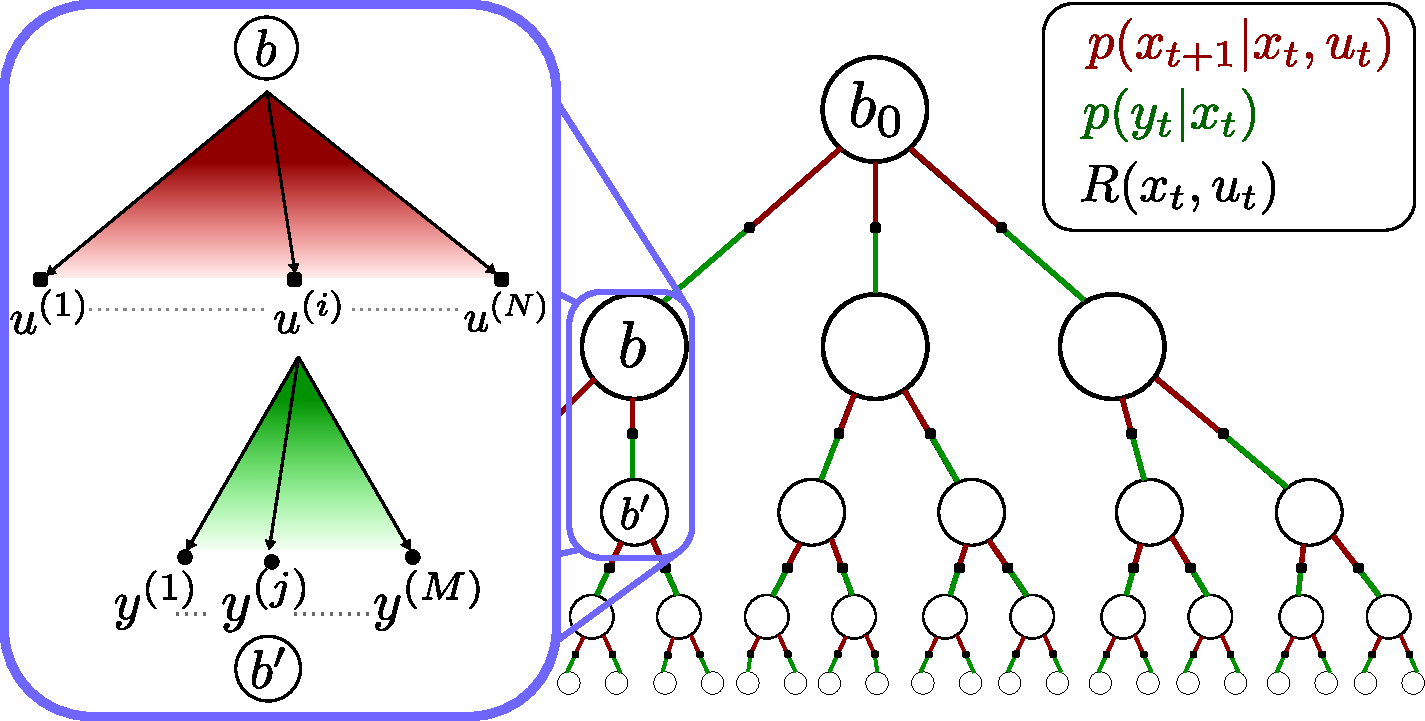
\includegraphics[width=0.8\textwidth]{/home/guillaume/Documents/Thesis/ch2-Background/Figures/belief_tree.pdf}
  \caption{ad}
\end{figure}

